\def\fpn{
    Các kiến trúc backbone \index{backbone} như AlexNet \index{AlexNet} \cite{krizhevsky2012imagenet}, VGG \index{VGG} \cite{simonyan2014very}, InceptionNet \index{InceptionNet} \cite{szegedy2015going}, SqueezeNet \index{SqueezeNet} \cite{iandola2016squeezenet} và đặc biệt là ResNet \index{ResNet} \cite{he2016deep} đã đạt những thành công nhất định.
    Tuy nhiên, các kiến trúc backbone \index{backbone} trên vẫn gặp phải một vấn đề về chênh lệch kích thước giữa các đối tượng trong ảnh.
    Feature Pyramid Networks \index{Feature Pyramid Networks} \cite{lin2017feature} (gọi tắt là FPN \index{FPN}) được giới thiệu như một kiến trúc backbone \index{backbone} nhằm giải quyết vấn đề trên.
    Việc sử dụng FPN \index{FPN} như là kiến trúc backbone \index{backbone} kết hợp cùng mô hình Faster R-CNN \index{Faster R-CNN} \index{Faster R-CNN} \cite{ren2015faster} đã vượt qua rất nhiều các mô hình nhận diện đối tượng \index{nhận diện đối tượng} khác để trở thành mô hình tốt nhất ở thời điểm đó.

    \noindent
    \textbf{\textit{So sánh các kiến trúc pyramid \index{kiến trúc pyramid} khác nhau}}

    \begin{figure}[H]
        \centering
        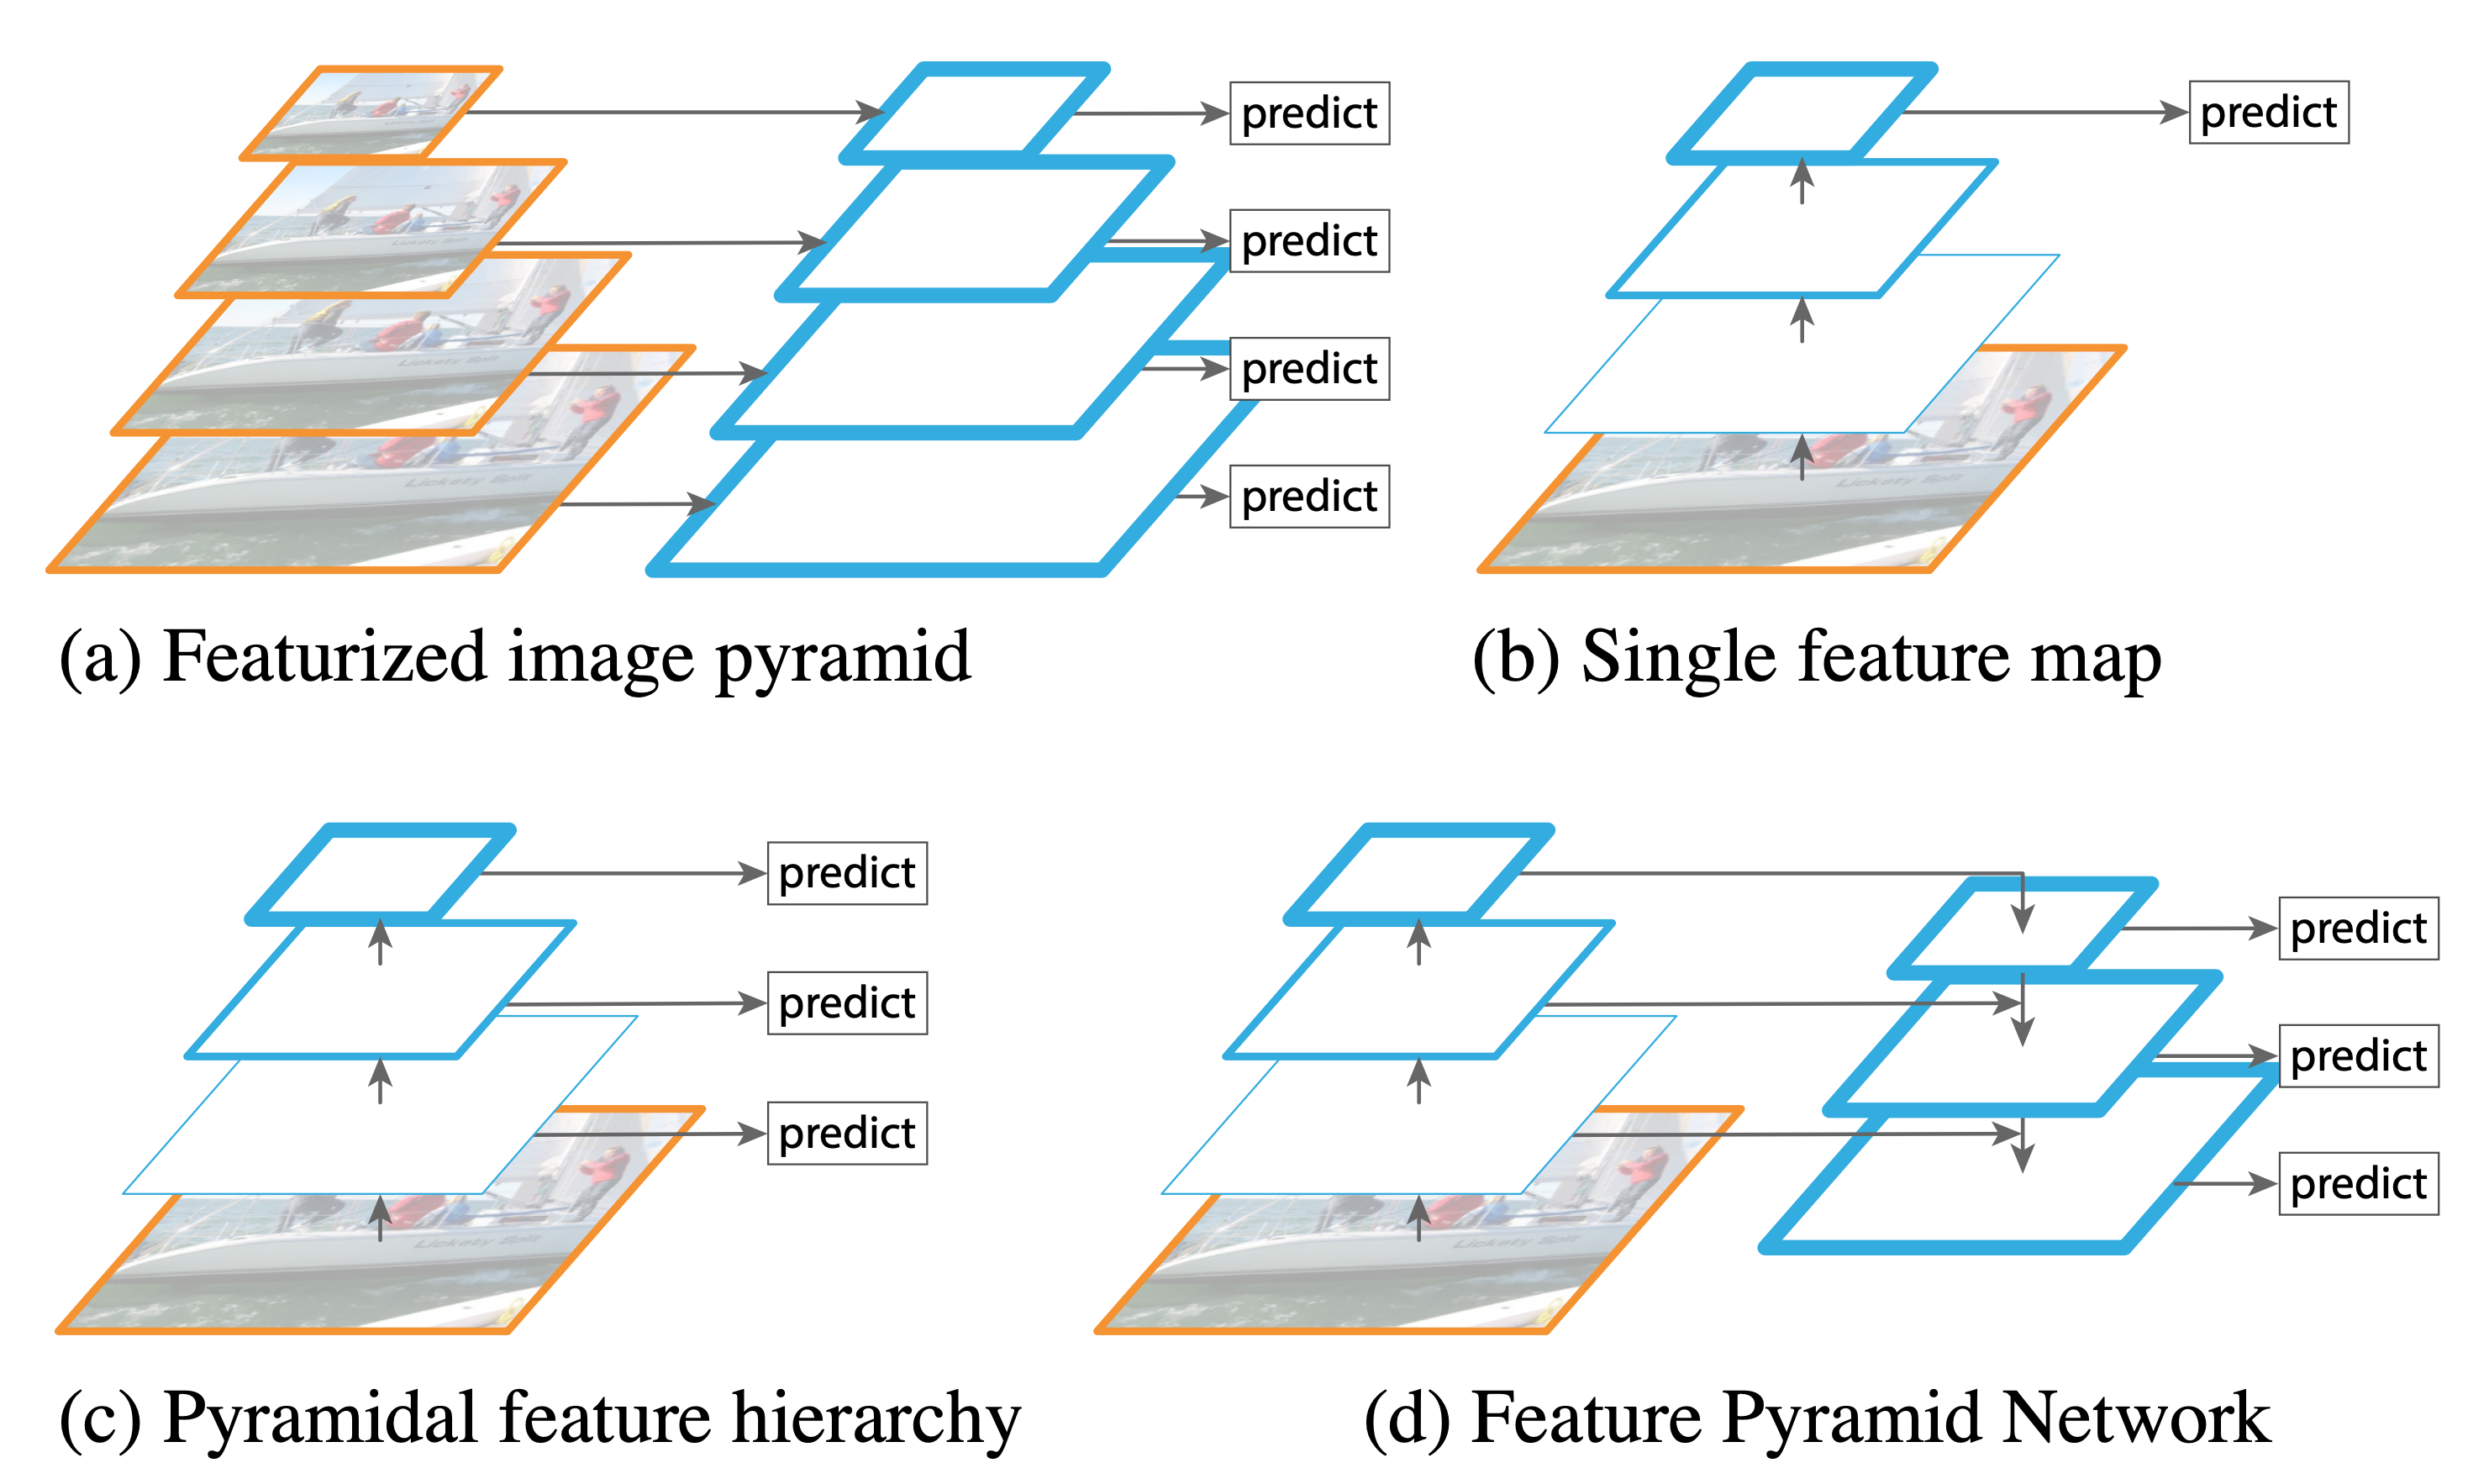
\includegraphics[width=11cm] {images/fpn_compare}
        \caption{So sánh các kiến trúc pyramid \index{kiến trúc pyramid} khác nhau (Nguồn: \cite{lin2017feature})}
        \label{fig:fpn_compare}
    \end{figure}

    \noindent
    Ý tưởng về việc xây dựng và sử dụng các đặc trưng của ảnh với nhiều kích thước khác nhau không mới, tuy nhiên, các giải pháp đã có vào thời điểm đó đều vướng phải một số vấn đề: \\
    - \textit{Featurized image pyramid} \index{Featurized image pyramid}: Việc sử dụng nhiều kích thước ảnh khác nhau để tạo ra nhiều đặc trưng có kích thước khác nhau một cách độc lập là ý tưởng cơ bản nhất. Mặc dù đạt được hiệu quả cao về độ chính xác khi khai thác ảnh đầu vào với nhiều kích thước khác nhau, nhưng phương pháp này khiến cho mô hình giải bài toán nhận diện đối tượng \index{nhận diện đối tượng} trở nên cồng kềnh và tốn rất nhiều thời gian để xử lý và gần như bất khả thi để có thể train được mô hình. \\
    - \textit{Single feature map} \index{Single feature map}: Việc sử dụng chỉ một kích thước đặc trưng duy nhất giúp cho mô hình xử lý nhanh hơn nhưng lại khiến cho mô hình khó có thể học được những đặc trưng giữa các đối tượng có kích thước chênh lệch trong ảnh. Đặc biệt, việc đưa ảnh đầu vào qua nhiều khối Conv đã loại bỏ rất nhiều thông tin và gần như không còn thông tin để mô hình có thể nhận biết được các đối tượng có kích thước nhỏ. \\
    - \textit{Pyramidal feature hierarchy} \index{Pyramidal feature hierarchy}: Việc sử dụng nhiều feature maps \index{feature maps} có kích thước khác nhau cùng đưa ra kết quả được sử dụng trong mô hình nhận diện đối tượng \index{nhận diện đối tượng} khá nổi tiếng là SSD \index{SSD} \cite{liu2016ssd}. Tuy nhiên, thay vì tận dụng toàn bộ các feature maps \index{feature maps} sinh ra từ các khối Conv của backbone \index{backbone} VGG-16 \index{VGG-16}, SSD \index{SSD} chỉ sử dụng feature maps \index{feature maps} từ khối Conv thứ 5 và bổ sung thêm các lớp Conv \index{lớp Conv}. Điều này khiến cho SSD \index{SSD} bỏ qua những feature maps \index{feature maps} có kích thước lớn, có ý nghĩa quan trọng trong việc detect các đối tượng có kích thước nhỏ. \\
    - \textit{Feature Pyramid Network} \index{Feature Pyramid Network}: Dựa trên vấn đề trên từ SSD \index{SSD}, nhóm tác giả đề xuất FPN \index{FPN} tận dụng tối đa các feature maps \index{feature maps} trích xuất được từ backbone \index{backbone} nhằm tạo ra bộ feature maps \index{feature maps} mới gồm nhiều kích thước khác nhau và chứa rất nhiều thông tin về nội dung của ảnh đầu vào. Để đạt được điều này, nhóm tác giả thiết kế kiến trúc kết hợp những feature maps \index{feature maps} có kích thước lớn và những feature maps \index{feature maps} có kích thước nhỏ bằng top-down pathway \index{top-down pathway} và lateral connections \index{lateral connections}.

    \noindent
    \textbf{\textit{Kiến trúc mô hình Feature Pyramid Networks}} \\
    Ý tưởng về việc sử dụng kiến trúc mô hình theo dạng top-down không phải là mới và đã được nhắc đến trong một số nghiên cứu. Tuy nhiên, điểm giống nhau của các nghiên cứu có thiết kế mô hình theo kiểu top-down đó là mô hình chỉ sử dụng một feature maps \index{feature maps} cuối cùng, sau khi đã tổng hợp các thông tin trong suốt quá trình top-down, để đưa ra quyết định dự đoán cuối cùng.

    \noindent
    Trong khi đó, đối với FPN, nhóm tác giả đưa ra quyết định dự đoán trên từng feature maps \index{feature maps} trong suốt quá trình top-down. Từ đó, đặc biệt nâng cao chất lượng của mô hình nhận diện đối tượng \index{nhận diện đối tượng} khi có thể vừa trích xuất được thông tin của các đối tượng có kích thước lớn từ các feature maps \index{feature maps} có kích thước nhỏ vừa trích xuất được thông tin của các đối tượng có kích thước nhỏ từ các feature maps \index{feature maps} có kích thước lớn.

    \begin{figure}[H]
        \centering
        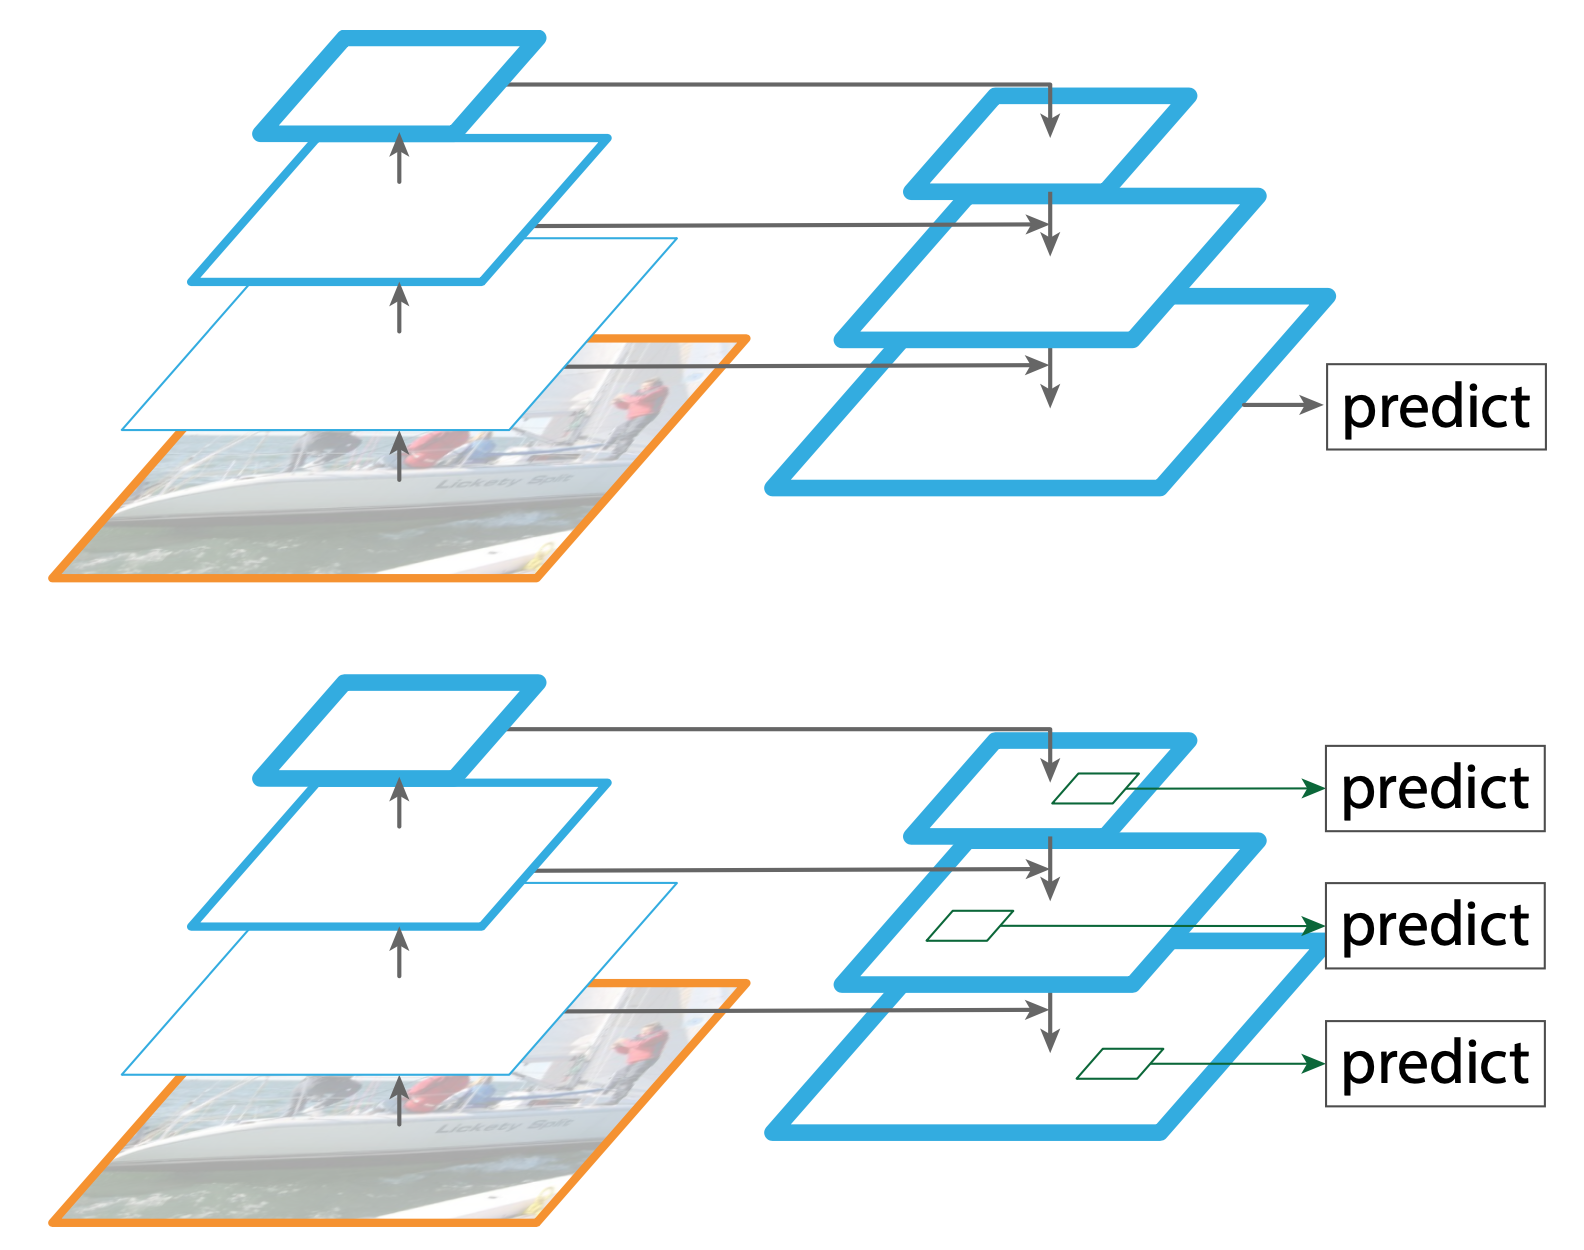
\includegraphics[width=6cm] {images/fpn_topdown}
        \caption{So sánh các kiến trúc theo dạng top-down khác nhau (Nguồn: \cite{lin2017feature})}
        \label{fig:fpn_topdown}
    \end{figure}

    \noindent
    Kiến trúc FPN \index{FPN} có thể được áp dụng với nhiều backbone \index{backbone} Conv khác nhau như AlexNet, VGG hay ResNet, cụ thể trong nghiên cứu, nhóm tác giả lựa chọn ResNet làm mô hình backbone.
    Kiến trúc FPN \index{FPN} có thể được chia làm hai phần: \\
    - \textit{Bottom-up pathway} \index{bottom-up pathway} là quá trình mà ta đưa ảnh đầu vào qua mô hình backbone \index{backbone} Conv như ResNet và thu được các feature maps \index{feature maps}.
    Tuy nhiên, trong các mô hình backbone \index{backbone} Conv, sẽ có một nhóm các lớp Conv \index{lớp Conv} tạo ra các feature maps \index{feature maps} có kích thước giống nhau, và nhóm các lớp Conv \index{lớp Conv} này được gọi là một khối Conv.
    Đối với FPN, nhóm tác giả lựa chọn các feature maps \index{feature maps} được sinh ra từ các lớp Conv \index{lớp Conv} cuối cùng trong mỗi khối Conv để sử dụng cho nhánh top-down pathway \index{top-down pathway}.
    Cụ thể đối với mô hình backbone \index{backbone} ResNet, nhóm tác giả sử dụng các feature maps \index{feature maps} được sinh ra từ residual block cuối cùng của mỗi khối Conv (trừ khối Conv đầu tiên do kích thước của feature maps \index{feature maps} này lớn và gây ra vấn đề về bộ nhớ), ký hiệu là \textit{{${C}_{2}, {C}_{3}, {C}_{4}, {C}_{5}$}}.
    Các feature maps \index{feature maps} này có kích thước lần lượt bằng 1/4, 1/8, 1/16 và 1/32 so với kích thước của ảnh đầu vào. \\
    - \textit{Top-down pathway và lateral connections} \index{top-down pathway} \index{lateral connections} là quá trình mà FPN \index{FPN} sinh ra thêm các feature maps \index{feature maps} mới từ các feature maps \index{feature maps} của bottom-up pathway \index{bottom-up pathway} và kết hợp chúng lại thông qua lateral connections \index{lateral connections}.
    Cụ thể, các feature maps \index{feature maps} của bottom-up pathway \index{bottom-up pathway} được đưa qua các lớp Conv \index{lớp Conv} có kích thước 1x1, stride \index{stride} bằng 1 nhằm giữ nguyên kích thước chiều dài, chiều rộng và chỉ thay đổi kích thước chiều channel \index{channel} của feature maps \index{feature maps}.
    Các feature maps \index{feature maps} ở vị trí cao hơn (có kích thước nhỏ hơn) được upsample \index{upsample} thông qua thuật toán nearest neighbor \index{nearest neighbor} và cộng ma trận với feature maps \index{feature maps} đầu ra từ lớp Conv \index{lớp Conv} 1x1 nói trên.
    Cuối cùng, các feature maps \index{feature maps} đầu ra từ phép cộng ma trận nói trên được đi qua một lớp Conv \index{lớp Conv} 3x3 có cùng số đầu ra channel \index{channel} của feature maps \index{feature maps} nhằm giảm bớt hiệu ứng của thuật toán nearest neighbor \index{nearest neighbor} và tạo ra các feature maps \index{feature maps} đầu ra cuối cùng có cùng số channel \index{channel} với nhau.
    Tập hợp feature maps \index{feature maps} này được gọi là \textit{{${P}_{2}, {P}_{3}, {P}_{4}, {P}_{5}$}} tương ứng với các feature maps \index{feature maps} có cùng kích thước \textit{{${C}_{2}, {C}_{3}, {C}_{4}, {C}_{5}$}}.

    \begin{figure}[H]
        \centering
        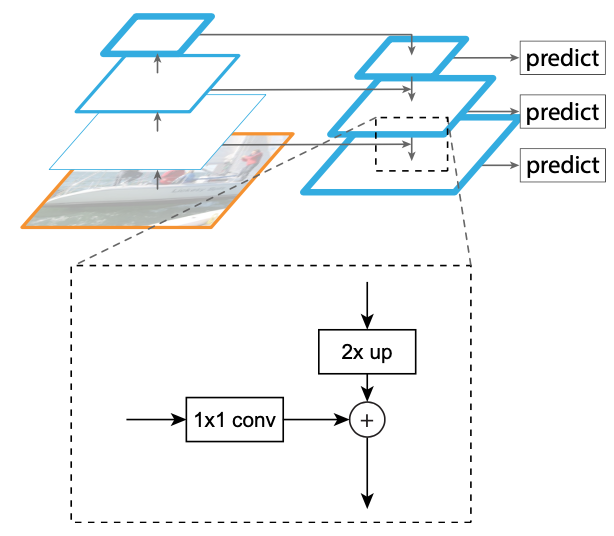
\includegraphics[width=6cm] {images/fpn_detail}
        \caption{Chi tiết kiến trúc FPN (Nguồn: \cite{lin2017feature})}
        \label{fig:fpn_detail}
    \end{figure}

    \noindent
    \textbf{\textit{Sử dụng kiến trúc FPN cho mô hình RPN}} \\
    Ý tưởng về việc sử dụng kiến trúc FPN \index{FPN} cho mô hình RPN \index{RPN} \cite{ren2015faster} được nhóm tác giả đề xuất nhằm cải thiện khả năng đề xuất ra các khu vực có kích thước chênh lệch nhau.
    Cụ thể, thay vì việc sử dụng một feature maps \index{feature maps} thu được từ feature extraction module \index{feature extraction module}, nhóm tác giả sử dụng các feature maps \index{feature maps} \textit{{${P}_{2}, {P}_{3}, {P}_{4}, {P}_{5}, {P}_{6}$}} (nhóm tác giả sử dụng thêm feature maps \index{feature maps} ${P}_{6}$ nhằm đề xuất ra những khu vực có kích thước lớn hơn).
    Các feature maps \index{feature maps} này cùng được đưa qua một bộ các lớp Conv \index{lớp Conv} 3x3 và 1x1 chung để trả đầu ra kết quả anchor \index{anchor} có chứa đối tượng hay không và toạ độ của khu vực mà mô hình đề xuất.
    Với việc sử dụng nhiều feature maps \index{feature maps} có các kích thước khác nhau, trên mỗi feature maps \index{feature maps}, nhóm tác giả chỉ sử dụng một kích thước anchor \index{anchor} lần lượt tương ứng \textit{{${32}^{2}, {64}^{2}, {128}^{2}, {256}^{2}, {512}^{2},$}} với ba tỷ lệ chiều dài giữa chiều rộng là \textit{1:2, 1:1, 2:1}.
    Để có thể train được, nhóm tác giả cũng sử dụng cơ chế gán positive/negative anchor \index{anchor} tương tự như chiến lược được đề xuất trong \cite{ren2015faster}.

    \begin{figure}[H]
        \centering
        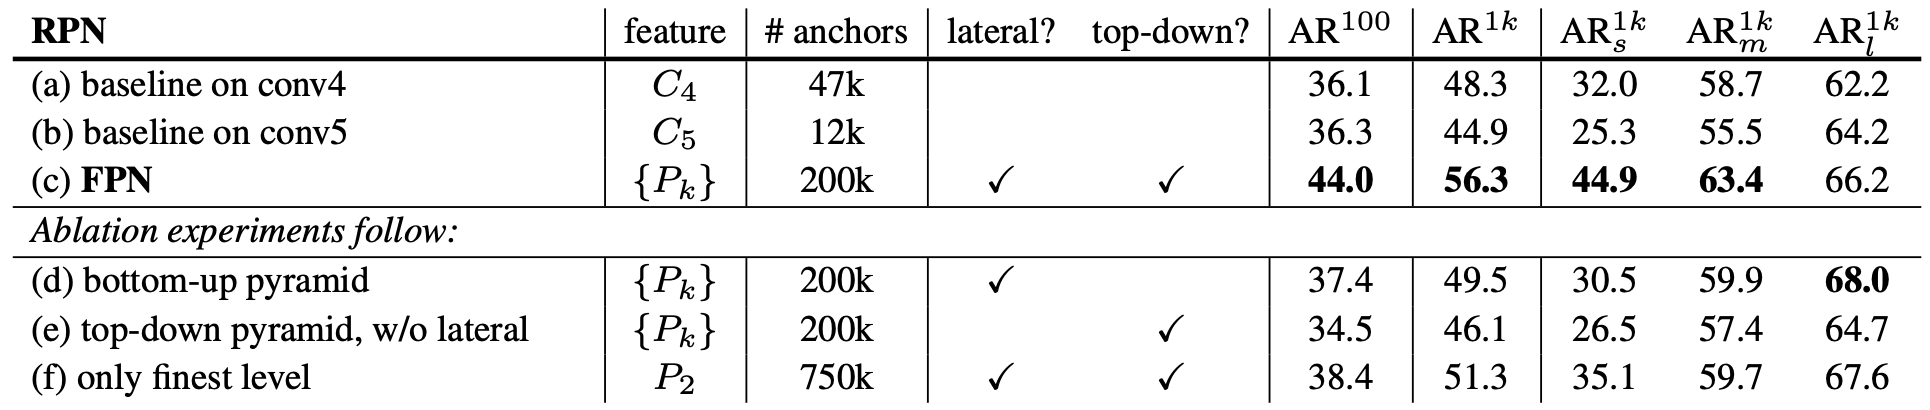
\includegraphics[width=12cm] {images/fpn_results_1}
        \caption{Kết quả của thí nghiệm sử dụng kiến trúc FPN cho mô hình RPN \index{RPN} \cite{ren2015faster} (Nguồn: \cite{lin2017feature})}
        \label{fig:fpn_results}
    \end{figure}

    \noindent
    Kết quả của thí nghiệm sử dụng kiến trúc FPN \index{FPN} cho mô hình RPN \index{RPN} \cite{ren2015faster} được nhóm tác giả chia sẻ khá khả quan.
    Ngoài việc so sánh việc sử dụng kiến trúc FPN \index{FPN} với các kiến trúc trước đây của mô hình RPN, nhóm tác giả còn so sánh thêm một số cấu hình khác của kiến trúc FPN \index{FPN}.
    Cụ thể các cấu hình như sau: \\
    - \textit{baseline on conv4} là cấu hình sử dụng feature maps \index{feature maps} từ lớp Conv \index{lớp Conv} thứ 4 của feature extraction module \index{feature extraction module} cho mô hình RPN. \\
    - \textit{baseline on conv5} là cấu hình sử dụng feature maps \index{feature maps} từ lớp Conv \index{lớp Conv} thứ 5 của feature extraction module \index{feature extraction module} cho mô hình RPN. \\
    - \textit{FPN} là cấu hình sử dụng kiến trúc FPN trích xuất các feature maps \index{feature maps} cho mô hình RPN. \\
    - \textit{bottom-up pyramid} là cấu hình sử dụng các feature maps \index{feature maps} \textit{{${P}_{2}, {P}_{3}, {P}_{4}, {P}_{5}, {P}_{6}$}} cho mô hình RPN.
    Tuy nhiên, giữa các feature maps \index{feature maps} này không có top-down pathway với nhau (hay nói cách khác, các feature maps \index{feature maps} \textit{{${P}_{2}, {P}_{3}, {P}_{4}, {P}_{5}, {P}_{6}$}} được sinh một cách độc lập từ các feature maps \index{feature maps} \textit{{${C}_{2}, {C}_{3}, {C}_{4}, {C}_{5}, {C}_{6}$}}). \\
    - \textit{top-down pyramid, w/o lateral} là cấu hình sử dụng các feature maps \index{feature maps} \textit{{${P}_{2}, {P}_{3}, {P}_{4}, {P}_{5}, {P}_{6}$}} cho mô hình RPN.
    Tuy nhiên, giữa các feature maps \index{feature maps} \textit{{${P}_{3}, {P}_{4}, {P}_{5}, {P}_{6}$}} không có lateral connections \index{lateral connections} với các feature maps \index{feature maps} \textit{{${C}_{3}, {C}_{4}, {C}_{5}, {C}_{6}$}} (hay nói cách khác, các feature maps \index{feature maps} \textit{{${P}_{3}, {P}_{4}, {P}_{5}, {P}_{6}$}} chỉ được sinh từ các feature maps \index{feature maps} \textit{{${P}_{2}, {P}_{3}, {P}_{4}, {P}_{5}$}}). \\
    - \textit{only finest level} là cấu hình chỉ sử dụng duy nhất feature maps \index{feature maps} \textit{${P}_{2}$} cho mô hình RPN. \\
    Trong đó, tất cả các cấu hình được train với bộ dữ liệu \textit{COCO trainval135k} và kết quả thu được đánh giá trên bộ dữ liệu \textit{COCO minival}.
    feature maps \index{feature maps} sử dụng trong cấu hình được ghi chú tại cột \textbf{feature}, số lượng khu vực được đề xuất trong quá trình test được thống kê tại cột \textbf{\# anchors}, cấu hình có sử dụng lateral connections \index{lateral connections} và top-down pathway hay không được chú thích tại cột \textbf{lateral} và \textbf{top-down}. \\
    Cấu hình \textit{FPN} đạt kết quả cao hơn vượt trội so với các cấu hình \textit{baseline on conv4} và \textit{baseline on conv5} nguyên bản.
    Cấu hình \textit{FPN} chỉ đạt kết quả kém hơn so với cấu hình \textit{bottom-up pyramid} khi so sánh trên chỉ số đánh giá với những bounding box \index{bounding box} có kích thước lớn, tuy nhiên, sự chênh lệch giữa hai cấu hình là không quá khác biệt.

    \noindent
    \textbf{\textit{Sử dụng kiến trúc FPN cho mô hình Fast R-CNN \index{Fast R-CNN}}} \\
    Ý tưởng về việc sử dụng kiến trúc FPN cho mô hình Fast R-CNN \index{Fast R-CNN} được nhóm tác giả đề xuất nhằm cải thiện khả năng định vị ra bounding box \index{bounding box} từ các khu vực đã được đề xuất từ mô hình RPN.
    Cụ thể, sau khi đưa ảnh qua region proposals module \index{region proposals module} của mô hình Fast R-CNN \index{Fast R-CNN} là Selective Search, ta thu được toạ độ của khu vực được đề xuất trên ảnh đầu vào.
    Đối với mô hình Fast R-CNN \index{Fast R-CNN} nguyên bản, ta dễ dàng lấy được khu vực đề xuất trên feature maps \index{feature maps} của ảnh đầu vào, tuy nhiên, với việc sử dụng kiến trúc FPN cho feature extraction module \index{feature extraction module}, câu hỏi đặt ra là đối với từng khu vực đề xuất ta xác định feature maps \index{feature maps} nào trong số \textit{{${P}_{2}, {P}_{3}, {P}_{4}, {P}_{5}$}} để lấy làm đầu vào cho lớp RoI pooling?
    Nhóm tác giả đã coi danh sách feature maps \index{feature maps} \textit{{${P}_{2}, {P}_{3}, {P}_{4}, {P}_{5}$}} sinh ra bởi FPN tương tự với các feature maps \index{feature maps} được sinh ra từ việc sử dụng image pyramids và áp dụng công thức sau để xác định feature maps \index{feature maps} phù hợp cho từng khu vực làm đầu vào của lớp RoI pooling.

    \begin{equation}
        \label{eq:roi_mapping}
        k = \lfloor k_0 + \log_2(\sqrt{wh} / 224) \rfloor.
    \end{equation}

    \noindent
    trong đó: \\
    \textit{k} là index của feature maps \index{feature maps} sử dụng làm đầu vào cho lớp RoI pooling tương ứng với khu vực đề xuất có kích thước chiều rộng là \textit{w} và chiều cao là \textit{h} \\
    $k_0$ là index của feature maps \index{feature maps} sử dụng làm đầu vào cho lớp RoI pooling tương ứng với khu vực đề xuất có kích thước chiều rộng và chiều cao lần lượt là 224 và 224 \\
    Tác giả lựa chọn con số 224 bởi đây là kích thước ảnh của pretrained ImageNet và lựa chọn $k_0 = 4$. \\
    Các feature maps \index{feature maps} được lấy ra tương ứng với từng khu vực đề xuất được đưa qua lớp lớp RoI pooling có kích thước đầu ra là 7x7 và được đưa qua chung các lớp Conv \index{lớp Conv} và lớp fully connected \index{lớp fully connected} để xác định lớp của đối tượng và toạ độ của bounding box \index{bounding box}.

    \begin{figure}[H]
        \centering
        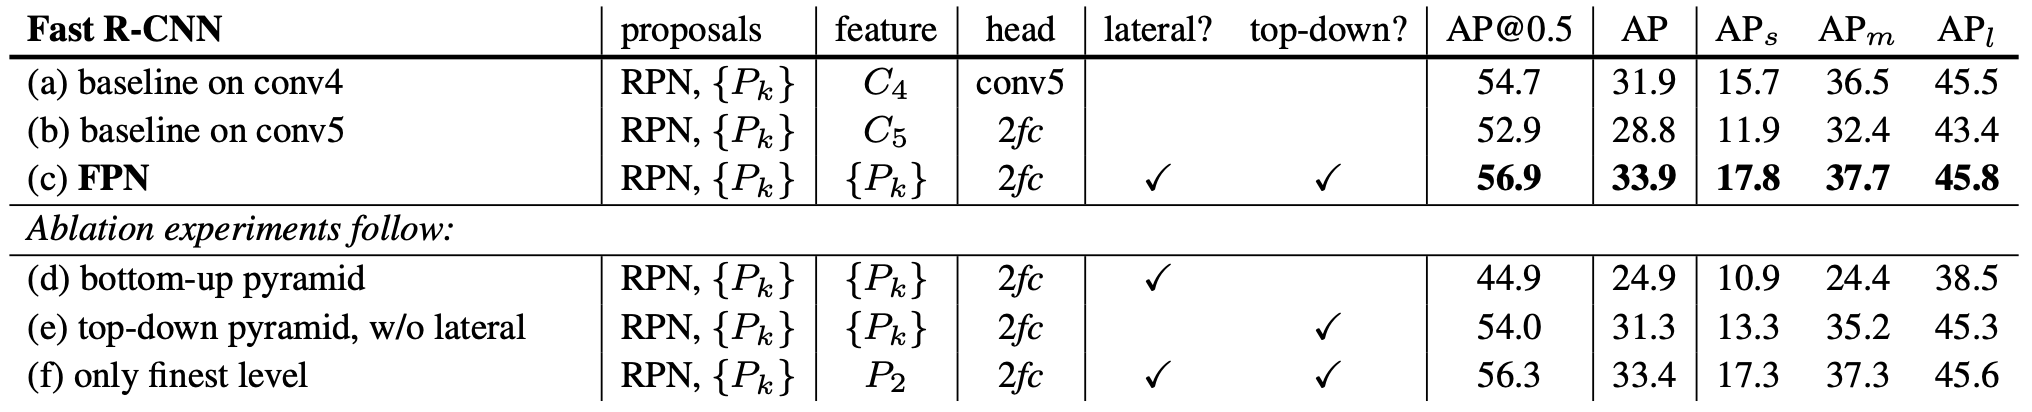
\includegraphics[width=12cm] {images/fpn_results_2}
        \caption{Kết quả của thí nghiệm sử dụng kiến trúc FPN cho mô hình Fast R-CNN \index{Fast R-CNN} (Nguồn: \cite{lin2017feature})}
        \label{fig:fpn_results}
    \end{figure}
    
    \noindent
    Kết quả của thí nghiệm sử dụng kiến trúc FPN cho mô hình Fast R-CNN \index{Fast R-CNN} được nhóm tác giả chia sẻ khá ấn tượng.
    Ngoài việc so sánh việc sử dụng kiến trúc FPN với các kiến trúc trước đây của mô hình Fast R-CNN \index{Fast R-CNN}, nhóm tác giả còn so sánh thêm một số cấu hình khác của kiến trúc FPN.
    Cụ thể các cấu hình như sau: \\
    - \textit{baseline on conv4} là cấu hình sử dụng feature maps \index{feature maps} từ lớp Conv \index{lớp Conv} thứ 4 của feature extraction module \index{feature extraction module} cho mô hình Fast R-CNN \index{Fast R-CNN}. \\
    - \textit{baseline on conv5} là cấu hình sử dụng feature maps \index{feature maps} từ lớp Conv \index{lớp Conv} thứ 5 của feature extraction module \index{feature extraction module} cho mô hình Fast R-CNN \index{Fast R-CNN}. \\
    - \textit{FPN} là cấu hình sử dụng kiến trúc FPN trích xuất feature maps \index{feature maps} cho mô hình Fast R-CNN \index{Fast R-CNN} như mô tả ở trên. \\
    - \textit{bottom-up pyramid} là cấu hình sử dụng các feature maps \index{feature maps} \textit{{${P}_{2}, {P}_{3}, {P}_{4}, {P}_{5}, {P}_{6}$}} cho mô hình Fast R-CNN \index{Fast R-CNN}.
    Tuy nhiên, giữa các feature maps \index{feature maps} này không có top-down pathway với nhau (hay nói cách khác, các feature maps \index{feature maps} \textit{{${P}_{2}, {P}_{3}, {P}_{4}, {P}_{5}, {P}_{6}$}} được sinh một cách độc lập từ các feature maps \index{feature maps} \textit{{${C}_{2}, {C}_{3}, {C}_{4}, {C}_{5}, {C}_{6}$}}). \\
    - \textit{top-down pyramid, w/o lateral} là cấu hình sử dụng các feature maps \index{feature maps} \textit{{${P}_{2}, {P}_{3}, {P}_{4}, {P}_{5}, {P}_{6}$}} cho mô hình Fast R-CNN \index{Fast R-CNN}.
    - \textit{only finest level} là cấu hình chỉ sử dụng duy nhất feature maps \index{feature maps} \textit{${P}_{2}$} cho mô hình Fast R-CNN \index{Fast R-CNN}. \\
    Trong đó, tất cả các cấu hình được train với bộ dữ liệu \textit{COCO trainval135k} và kết quả thu được đánh giá trên bộ dữ liệu \textit{COCO minival} và cùng sử dụng chung một bộ khu vực đề xuất từ mô hình RPN.
    feature maps \index{feature maps} sử dụng trong cấu hình được ghi chú tại cột \textbf{feature}, kiến trúc mô hình RPN \index{RPN} \cite{ren2015faster} sử dụng trong từng cấu hình được chú thích tại cột \textbf{proposals}, cấu hình của phần head của mô hình Fast R-CNN \index{Fast R-CNN} được chú thích tại cột \textbf{head}, cấu hình có sử dụng lateral connections \index{lateral connections} và top-down pathway hay không được chú thích tại cột \textbf{lateral} và \textbf{top-down}. \\
    Cấu hình \textit{FPN} đạt kết quả cao hơn vượt trội so với các cấu hình \textit{baseline on conv4}, \textit{baseline on conv5} nguyên bản và cả các cấu hình tuỳ chọn như \textit{bottom-up pyramid}, \textit{top-down pyramid, w/o lateral}, \textit{only finest level}.

    \noindent
    \textbf{\textit{Sử dụng kiến trúc FPN cho toàn bộ các thành phần của mô hình Faster R-CNN}} \\
    Nhóm tác giả còn thực hiện một thí nghiệm nữa với kiến trúc FPN khi sử dụng FPN chung cho toàn bộ cả mô hình RPN \index{RPN} \cite{ren2015faster} và mô hình Fast R-CNN \index{Fast R-CNN} (mô hình RPN \index{RPN} \cite{ren2015faster} và mô hình Fast R-CNN \index{Fast R-CNN} sử dụng chung một kiến trúc backbone \index{backbone} FPN) và cũng đạt kết quả tương đối tốt.

    \begin{figure}[H]
        \centering
        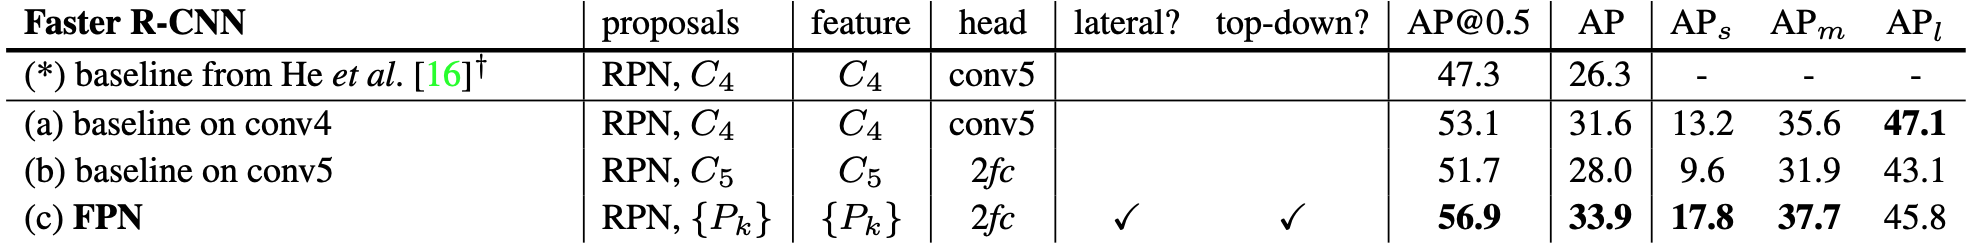
\includegraphics[width=12cm] {images/fpn_results_3}
        \caption{Kết quả của thí nghiệm sử dụng kiến trúc FPN cho mô hình Faster R-CNN \index{Faster R-CNN} (Nguồn: \cite{lin2017feature})}
        \label{fig:fpn_results_3}
    \end{figure}

    \noindent
    Cụ thể các cấu hình như sau: \\
    - \textit{baseline from He et al.} là mô hình ResNet được sử dụng cho bài toán nhận diện đối tượng \index{nhận diện đối tượng}. \\
    - \textit{baseline on conv4} là cấu hình sử dụng feature maps \index{feature maps} từ lớp Conv \index{lớp Conv} thứ 4 của feature extraction module \index{feature extraction module} cho cả hai nhánh của mô hình Faster R-CNN \index{Faster R-CNN}. \\
    - \textit{baseline on conv5} là cấu hình sử dụng feature maps \index{feature maps} từ lớp Conv \index{lớp Conv} thứ 5 của feature extraction module \index{feature extraction module} cho cả hai nhánh của mô hình Faster R-CNN \index{Faster R-CNN}. \\
    - \textit{FPN} là cấu hình sử dụng kiến trúc FPN trích xuất feature maps \index{feature maps} cho cả hai nhánh của mô hình Faster R-CNN \index{Faster R-CNN}. \\
    Trong đó, tất cả các cấu hình được train với bộ dữ liệu \textit{COCO trainval135k} và kết quả thu được đánh giá trên bộ dữ liệu \textit{COCO minival}.
    feature maps \index{feature maps} sử dụng trong cấu hình được ghi chú tại cột \textbf{feature}, kiến trúc mô hình RPN \index{RPN} \cite{ren2015faster} sử dụng trong từng cấu hình được chú thích tại cột \textbf{proposals}, cấu hình của phần head của mô hình Fast R-CNN \index{Fast R-CNN} được chú thích tại cột \textbf{head}, cấu hình có sử dụng lateral connections \index{lateral connections} và top-down pathway hay không được chú thích tại cột \textbf{lateral} và \textbf{top-down}. \\
    Cấu hình \textit{FPN} đạt kết quả cao hơn vượt trội so với các cấu hình còn lại trên hầu hết các chỉ số đánh giá.
    Chỉ có duy nhất chỉ số trên đối với các bounding box \index{bounding box} có kích thước lớn thì kết quả của cấu hình \textit{FPN} kém hơn một chút so với cấu hình \textit{baseline on conv4}.

    \noindent
    \textbf{\textit{Vấn đề tồn đọng của kiến trúc mô hình FPN}} \\
    Kiến trúc FPN ra đời đã tạo ra một trong số những kiến trúc backbone \index{backbone} kinh điển trong bài toán nhận diện đối tượng \index{nhận diện đối tượng} nói riêng.
    Kiến trúc FPN đã giúp cho nhiều mô hình đạt độ chính xác cao hơn và trong khi tốc độ của mô hình không bị tăng một cách đáng kể.
    Tuy nhiên, đối với cụ thể bài toán nhận diện đối tượng \index{nhận diện đối tượng}, việc kết hợp kiến trúc FPN vào mô hình Faster R-CNN \index{Faster R-CNN} mới chỉ cải thiện về mặt độ chính xác cho mô hình Faster R-CNN \index{Faster R-CNN} mà chưa giúp tăng tốc mô hình Faster R-CNN \index{Faster R-CNN}.
    Vẫn còn một câu hỏi cần phải được giải quyết đó là làm sao để duy trì được độ chính xác mà FPN mang lại những mô hình nhận diện đối tượng \index{nhận diện đối tượng} vẫn có để đạt tốc độ nhanh hơn nữa.
}